%% ------------------------------------------------------------------
%% Application Letter: ATLAS Software Development Grants 2027
%% Project 6: Update calorimeter clustering to support new (NN based
%% or similar) cell energy reconstruction
%%
%% Based on applications/_shared/latex/cover-letter-template.tex
%% Compile: latexmk -pdf cover-letter.tex
%%
%% Open TODOs are rendered in red (\todo{...}). Remove all before sending.
%% ------------------------------------------------------------------

\documentclass[11pt,a4paper]{article}

%% ------- Font and encoding (mirrors the CV) -------
\usepackage[utf8]{inputenc}
\usepackage[T1]{fontenc}
\usepackage[default]{lato}

%% ------- Layout -------
\usepackage[a4paper, top=1.5cm, bottom=1.75cm, left=2cm, right=2cm]{geometry}
\usepackage{parskip}
\setlength{\parindent}{0pt}
\setlength{\parskip}{0.7em}
\renewcommand{\baselinestretch}{1.12}

%% ------- Ragged right -------
\usepackage[document]{ragged2e}

%% ------- Hyperlinks -------
\PassOptionsToPackage{hyphens}{url}
\usepackage{hyperref}

%% ------- Shared visual identity -------
%% ------------------------------------------------------------------
%% identity.tex — Shared visual identity for CV and cover letters
%%
%% \input this file from any LaTeX document that should share the
%% Gonçalves visual identity (colors, icons, tipography helpers,
%% graphics search paths).
%%
%% Idempotent by design: safe to \input from documents that already
%% loaded xcolor / fontawesome / graphicx (via altacv or otherwise).
%% Uses \providecommand for macros so re-\input never errors.
%%
%% Callers currently include:
%%   - applications/_shared/latex/cover-letter-template.tex
%%   - applications/YYYY-MM-<slug>/cover-letter.tex (copied from template)
%%   - Optionally the CV itself, if the shared identity refactor is applied.
%% ------------------------------------------------------------------

%% ------- Required packages (loaded only if not already loaded) -------
\makeatletter
\@ifpackageloaded{xcolor}{}{\usepackage{xcolor}}
\@ifpackageloaded{fontawesome}{}{\usepackage{fontawesome}}
\@ifpackageloaded{graphicx}{}{\usepackage{graphicx}}
\@ifpackageloaded{tikz}{}{\usepackage{tikz}}
\makeatother

%% ------- Color palette (same values used by curriculum-en.tex) -------
\definecolor{StPatricksBlue}{HTML}{1F3D77}
\definecolor{SlateGrey}{HTML}{2E2E2E}
\definecolor{LightGrey}{HTML}{333333}

%% ------- Graphics search paths -------
%% Lets 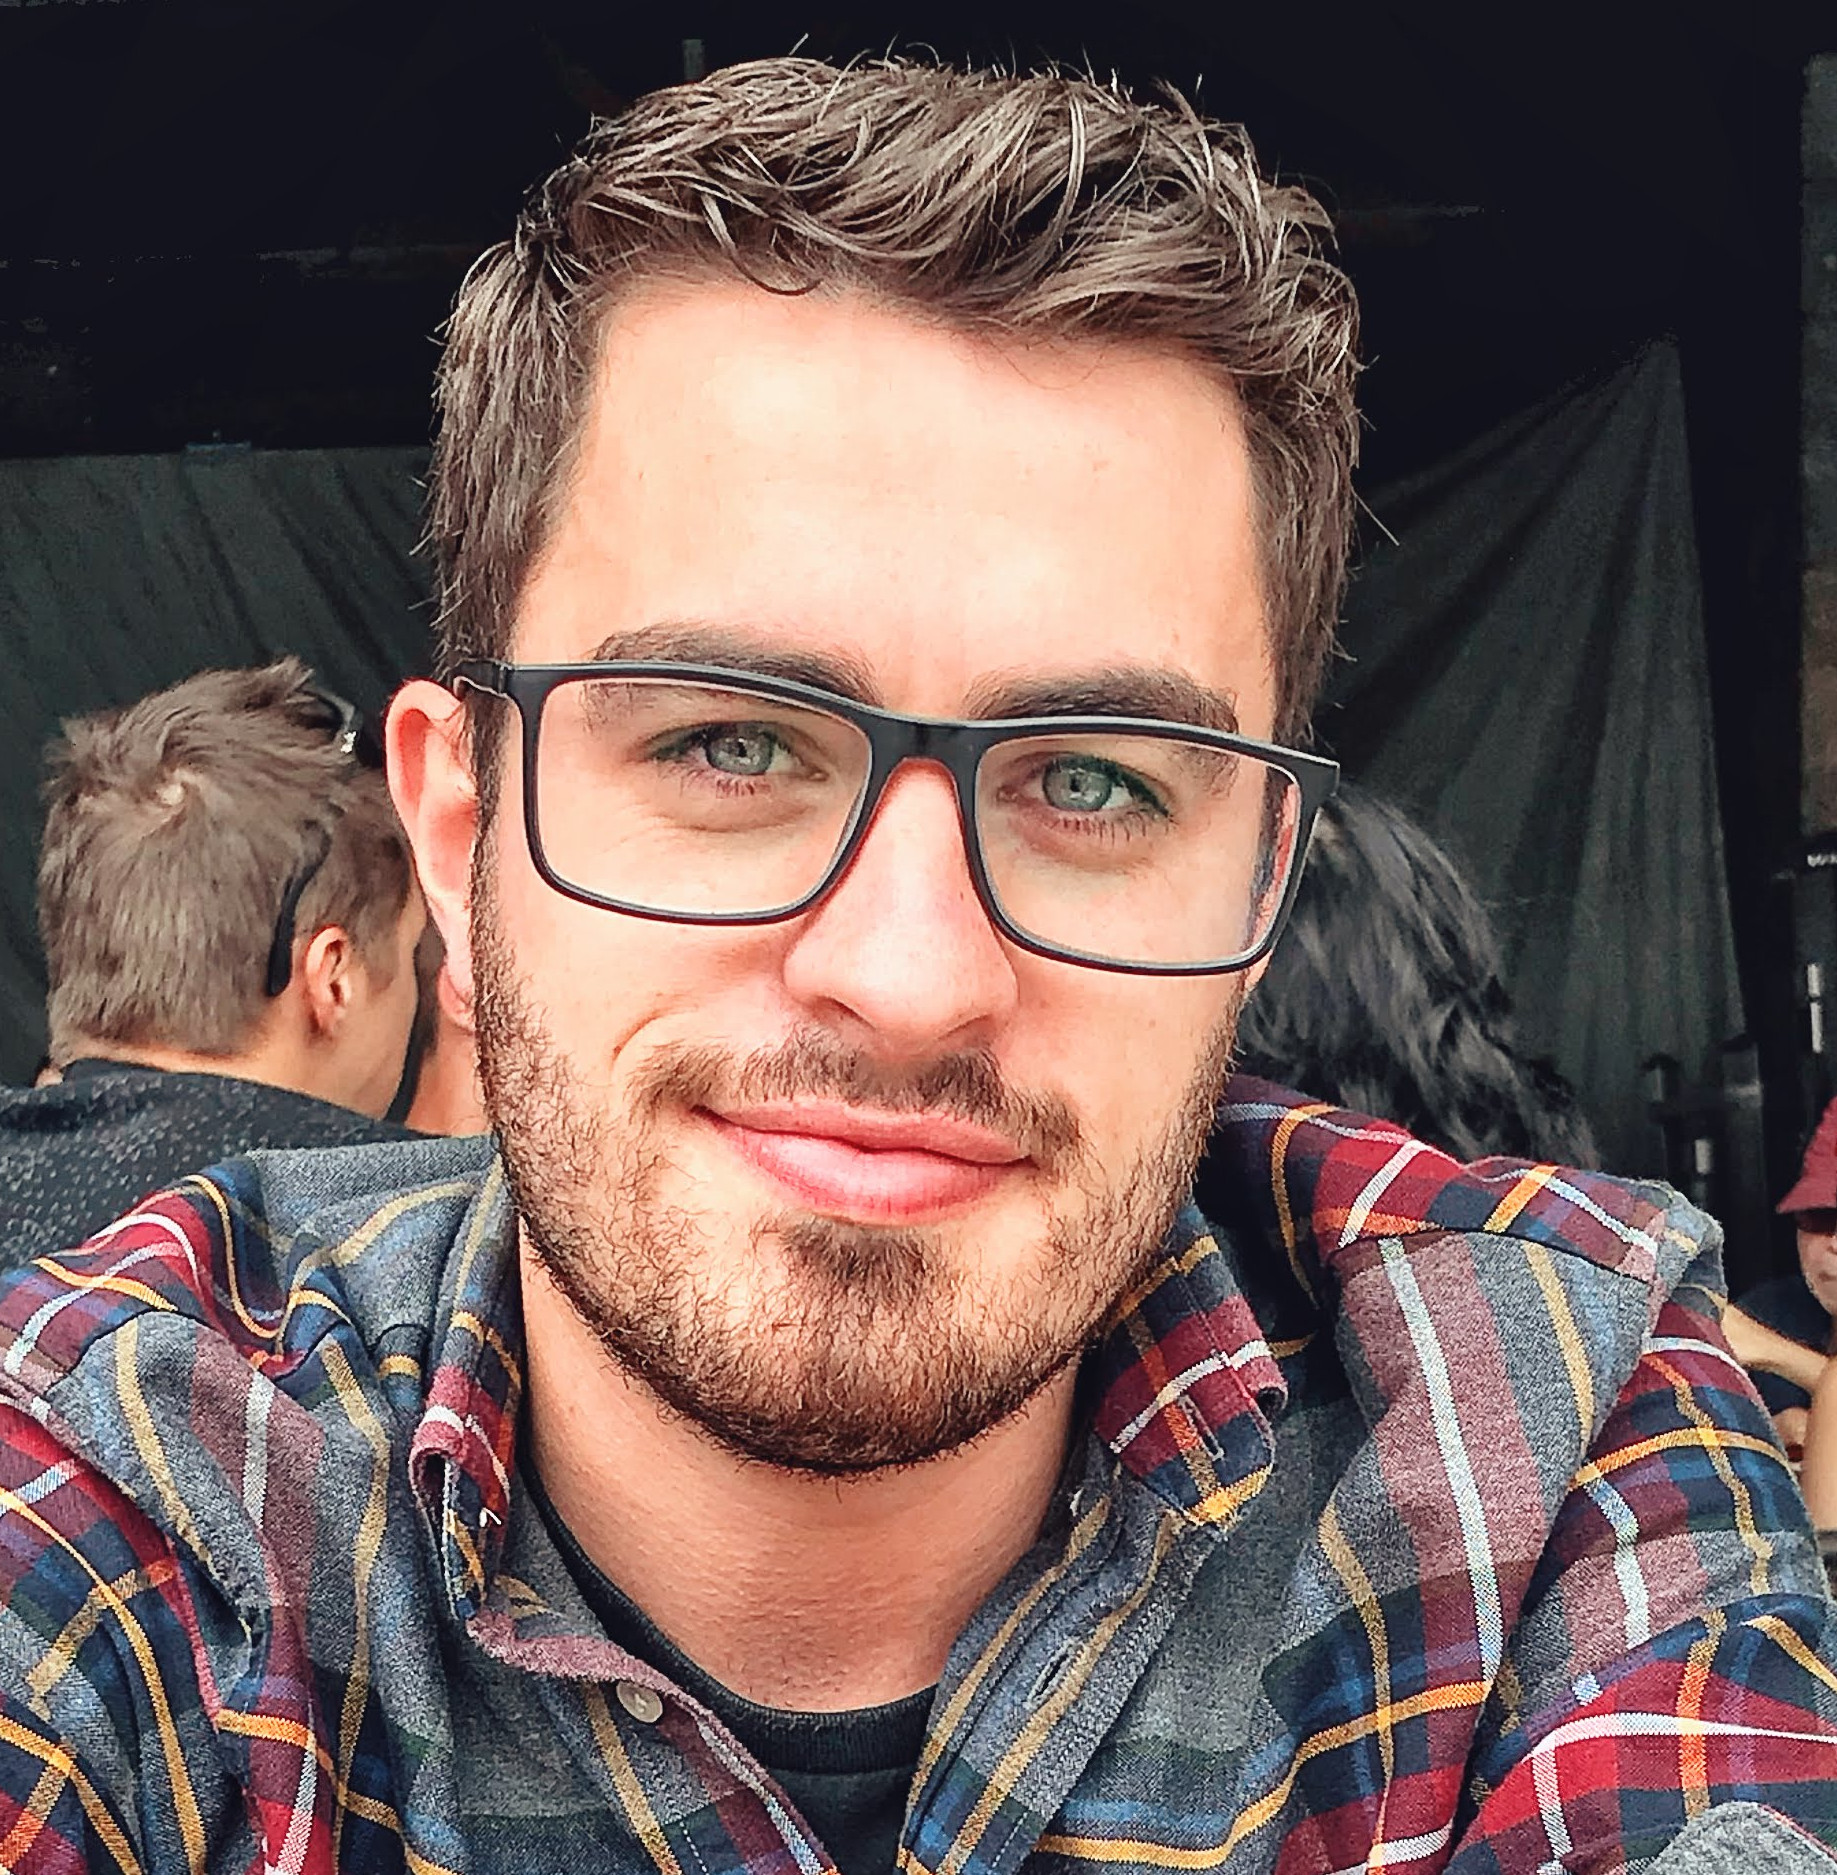
\includegraphics{profile} resolve to english/profile.jpg from any
%% depth the caller might be at. LaTeX tries these in order and uses the
%% first match.
\graphicspath{%
    {./}%                          same folder as the caller
    {./english/}%                  from project root
    {../english/}%                 from applications/ (unlikely, but cheap)
    {../../english/}%              from applications/YYYY-MM-<slug>/
    {../../../english/}%           from applications/_shared/latex/
}

%% ------- Style helpers for cover letters -------
%% Not used by the CV (altacv defines its own header macros), but harmless
%% to have loaded. \providecommand only defines if not already defined.

\providecommand{\senderName}[1]{%
    {\fontsize{22pt}{28pt}\selectfont\bfseries\color{StPatricksBlue}#1}%
}

\providecommand{\senderTagline}[1]{%
    {\fontsize{11pt}{14pt}\selectfont\itshape\color{SlateGrey}#1}%
}

\providecommand{\contactBullet}{%
    \hspace{0.5em}\textcolor{StPatricksBlue}{$\bullet$}\hspace{0.5em}%
}

\providecommand{\dividerLine}{%
    {\color{StPatricksBlue}\rule{\linewidth}{0.6pt}}%
}

\providecommand{\salutation}[1]{%
    {\bfseries\color{SlateGrey}#1}%
}

\providecommand{\closing}[1]{%
    {\bfseries\color{SlateGrey}#1}%
}

%% ------- Date and subject-line helpers for cover letters -------

%% \letterDate{City}
%% Renders "City, DD Month YYYY" right-aligned, in italic SlateGrey. Uses
%% \today under the hood so the date is always current at compile time.
%% Example: \letterDate{Lausanne}  ->  "Lausanne, 27 July 2026"
\providecommand{\letterMonth}{%
    \ifcase\month\or January\or February\or March\or April\or May\or June%
    \or July\or August\or September\or October\or November\or December\fi%
}
\providecommand{\letterDate}[1]{%
    \hfill{\itshape\color{SlateGrey}#1,~\the\day~\letterMonth~\the\year}%
}

%% \subjectLine{content}
%% Renders a bold SlateGrey subject line. Common convention in formal
%% European/Swiss/French letters (e.g. "Subject: ..." or "Object: ...").
%% The caller decides whether to include a prefix.
%% Example: \subjectLine{Subject: Application for Full Stack Engineer -- Ref. 2357}
\providecommand{\subjectLine}[1]{%
    {\bfseries\color{SlateGrey}#1}%
}

%% ------- Circular photo (matches altacv's \photo behavior in the CV) -------
%% \circularPhoto{diameter}{filename}
%% Renders a circular-cropped photo, resolving the filename via \graphicspath
%% (so \circularPhoto{2.5cm}{profile} finds english/profile.jpg).
%% The tikzpicture baseline is set to the top of the circle so that when used
%% inside a minipage with [t] alignment, the picture aligns with the top of
%% the row rather than the middle of the circle (default tikz behavior).
%% Example: \circularPhoto{2.5cm}{profile}
\providecommand{\circularPhoto}[2]{%
    \begin{tikzpicture}[baseline=(currentphoto.north)]
        \node[circle,minimum size=#1,inner sep=0pt,%
            path picture={%
                \node[inner sep=0pt] at (path picture bounding box.center) {%
                    \includegraphics[width=#1]{#2}%
                };%
            }%
        ] (currentphoto) {};
    \end{tikzpicture}%
}


\hypersetup{
    colorlinks=true,
    urlcolor=StPatricksBlue,
    linkcolor=StPatricksBlue,
    pdftitle={Guilherme I. Goncalves - Application - ATLAS Software Development Grants 2027},
    pdfauthor={Guilherme I. Goncalves}
}

%% Visible placeholder for facts still to be confirmed
\newcommand{\todo}[1]{{\color{red}\bfseries[TODO: #1]}}

\color{LightGrey}

%% ==================================================================
\begin{document}

%% ------- HEADER -------

\noindent%
\begin{minipage}[t]{\dimexpr\linewidth-3cm\relax}%
\senderName{Guilherme Inácio Gonçalves, Ph.D.}\\[0.4em]
\senderTagline{ATLAS Author, Rio de Janeiro State University (UERJ)}\\[0.8em]
{\color{LightGrey}\small
\faEnvelope\ \href{mailto:ginaciog@cern.ch}{ginaciog@cern.ch}\contactBullet%
\faPhone\ +55 22 99923 1446\contactBullet%
\faMapMarker\ Nova Friburgo, Brazil\\[0.3em]
CERN ID: 837130\contactBullet%
\faGithub\ \href{https://github.com/ingoncalves}{github.com/ingoncalves}
}%
\end{minipage}%
\hfill%
\begin{minipage}[t]{2.7cm}%
\circularPhoto{2.5cm}{profile}%
\end{minipage}%
\par

\vspace{0.75em}
\dividerLine
\vspace{1em}

%% ------- DATE -------

\letterDate{Nova Friburgo}

\vspace{0.5em}

%% ------- RECIPIENT BLOCK -------

{\color{SlateGrey}
ATLAS Software Development Grants Selection Committee\\
CERN, 1211 Geneva 23, Switzerland
}

\vspace{1em}

%% ------- SUBJECT LINE -------

\subjectLine{Subject: Application for the 2027 ATLAS Software Development Grants, Project 6}

\vspace{0.5em}

%% ------- SALUTATION -------

\salutation{Dear Members of the Selection Committee,}

%% ------- BODY -------

I am applying for the 2027 ATLAS Software Development Grants, with interest in Project~6, \emph{Update calorimeter clustering to support new (NN based or similar) cell energy reconstruction}. Enclosed are my CV and the supporting letter from the UERJ Institute Representatives. The project sits at the centre of my doctoral research: replacing optimal filtering with machine-learning-assisted cell energy reconstruction under HL-LHC pile-up, and understanding what that changes downstream.

\textbf{\color{SlateGrey}Experience and contributions to ATLAS}

I joined ATLAS in 2018 as a Master's student working on Tile Calorimeter energy reconstruction under high pile-up, supervised by Luciano Andrade and Bernardo Peralva. From 2019 to 2020 I worked on-site at CERN, implementing optimised digital Wiener filters in Athena, which led to an ATLAS conference paper (\href{https://cds.cern.ch/record/2752009/}{\nolinkurl{cds.cern.ch/record/2752009}}). In the same period I supported the Tile Muon Digitizer Board during LS2, served as a TileCal Data Quality validator, and led virtual ATLAS visits for public schools across Brazil.

My Ph.D. in Computational Modelling at UERJ, defended in February 2026, developed hybrid energy estimators for the HL-LHC TileCal readout: linear filters combined with a Multi-Layer Perceptron correction for pile-up, benchmarked against optimal filtering across cell occupancy regimes. I completed my qualification task on this topic in 2023 to 2024 and became an ATLAS author in 2024. The results are documented in a published TileCal Internal Note (\href{https://cds.cern.ch/record/2894828/}{\nolinkurl{cds.cern.ch/record/2894828}}).

Outside ATLAS, I developed the open-source \href{https://github.com/ingoncalves/calorimetry-pulse-simulator}{calorimetry-pulse-simulator} (C++ with Python bindings) and co-developed \href{https://github.com/lorenzetti-ufrj-br/lorenzetti}{Lorenzetti}, a general-purpose calorimetry simulation framework published in 2023. Both are used by other calorimetry groups for algorithm development and ML training. In parallel, I have more than eleven years of industry experience as a software engineer, currently Senior Full-Stack Engineer at Siteimprove and previously Technical Lead at O2 Filmes.

\textbf{\color{SlateGrey}Interest in Project 6}

The project asks for three things I have already worked on from different angles. First, the physics motivation: comparing NN-based cell energy reconstruction, and the pile-up noise information it provides, with optimal filtering is exactly the comparison my thesis made at the cell level; I would now carry it through to clustering and to electron and photon performance. Second, the software tasks: adding new per-cell information as decorations in \texttt{LArCellRec}, making it available to the \texttt{CaloRec} clustering algorithms behind a common configuration flag, keeping the optimal-filtering workflow bit-for-bit unchanged, and adding a CI test for the new data flow. Backward-compatible changes guarded by configuration, regression tests and CI are daily practice in my industry work, and my Athena experience means I can start productively, while learning the LAr and clustering code under the supervision of the project experts. Third, the follow-up: producing simulated Run-4 samples with the new reconstruction to support the e/$\gamma$ studies due by Summer 2028.

\textbf{\color{SlateGrey}Longer-term commitment}

I intend to stay with this work after the stay at CERN: completing the sample production and supporting the e/$\gamma$ studies through the Summer 2028 milestone, and then contributing to the maintenance of the clustering software for Run~4, from UERJ. The UERJ group has worked on calorimeter signal reconstruction in ATLAS for years, and the supporting letter describes how the institute will take up these topics with students from our Computational Modelling and Computer Engineering programmes.

Thank you for considering my application. I remain at your disposal for any further information.

\vspace{0.5em}

\closing{Sincerely,}

\vspace{1.5em}

\textbf{Guilherme I. Gonçalves, Ph.D.}\\
{\small ATLAS Author, Rio de Janeiro State University (UERJ), ATLAS/Brazil Cluster}

\end{document}
